\documentclass[convert={outext=.svg,density=750}]{standalone}
\usepackage{amsmath}

% More defined colors
\usepackage[dvipsnames]{xcolor}

% Required package
\usepackage{tikz}
\usetikzlibrary{positioning}
\usetikzlibrary{shapes.multipart}


\begin{document}

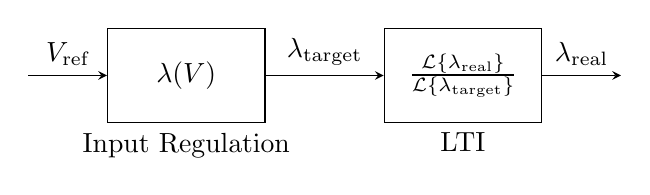
\begin{tikzpicture}[every text node part/.style={align=center}]

    % % Sum shape
    % \node[draw,
    %     circle,
    %     minimum size=0.6cm,
    %     fill=Rhodamine!50
    % ] (sum) at (0,0){};

    % \draw (sum.north east) -- (sum.south west)
    % (sum.north west) -- (sum.south east);

    % \node[left=-1pt] at (sum.center){\tiny $+$};
    % \node[below] at (sum.center){\tiny $-$};

    % % Controller
    % \node [draw,
    %     fill=Goldenrod,
    %     minimum width=2cm,
    %     minimum height=1.2cm,
    %     % right=1cm of sum
    % ]  (controller) at (0,0){$C(s)$};

    % % System H(s)
    % \node [draw,
    %     fill=SpringGreen,
    %     minimum width=2cm,
    %     minimum height=1.2cm,
    %     right=1.5cm of controller
    % ] (system) {$H(s)$};

    % % Sensor block
    % \node [draw,
    %     fill=SeaGreen,
    %     minimum width=2cm,
    %     minimum height=1.2cm,
    %     below right= 1cm and -0.25cm of controller
    % ]  (sensor) {$G(s)$};

    % Arrows with text label
    % \draw[-stealth] (sum.east) -- (controller.west)
    % node[midway,above]{$e$};

    % \draw[-stealth] (controller.east) -- (system.west)
    % node[midway,above]{$u$};

    % \draw[-stealth] (system.east) -- ++ (1.25,0)
    % node[midway](output){}node[midway,above]{$y$};

    % \draw[-stealth] (output.center) |- (sensor.east);

    % \draw[-stealth] (sensor.west) -| (sum.south)
    % node[near end,left]{$y_m$};

    % \draw (sum.west) -- ++(-1,0)
    % node[midway,above]{$y_{\text{ref}}$};

    % Input regulation
    \node [draw,
        minimum width=2cm,
        minimum height=1.2cm,
        label=below:Input Regulation
    ]  (input_regulation) at (0,0){$\lambda(V)$};

    % Wavelength Conversion
    \node [draw,
        minimum width=2cm,
        minimum height=1.2cm,
        label=below:LTI,
        right=1.5cm of input_regulation,
    ]  (LTI){$\frac{\mathcal{L}\{\lambda_\text{real}\}}{\mathcal{L}\{\lambda_\text{target}\}}$};

    % Arrows
    \node (foo)[left of=input_regulation]{};
    \draw[stealth-] (input_regulation.west) -- ++(-1,0)
    node[midway,above](){$V_\text{ref}$};

    \draw[-stealth] (input_regulation.east) -- (LTI.west)
    node[midway,above](){$\lambda_\text{target}$};

    \draw[-stealth] (LTI.east) -- ++(1,0)
    node[midway,above](){$\lambda_\text{real}$};


\end{tikzpicture}

\end{document}
